% cd /disks/PROJECT/Mickael/COMMUNICATION/IMIDIA/;
% pdflatex Beamer_IMIDIA.tex; bibtex Beamer_IMIDIA; pdflatex Beamer_IMIDIA.tex; pdflatex Beamer_IMIDIA.tex
% evince Beamer_IMIDIA.pdf &

% \documentclass[10pt, handout, xcolors={RGB}, hyperref={pdfpagelabels=false,
\documentclass[10pt, xcolors={RGB}, hyperref={pdfpagelabels=false,
        colorlinks=true,
        pdftex=true,
        bookmarks=true,
        bookmarksopen=true,
        hyperfootnotes=true}]{beamer}
\pdfpageattr{/Group << /S /Transparency /I true /CS /DeviceRGB>>}

\usepackage[T1]{fontenc}
\usepackage[utf8]{inputenc}
\usepackage{graphicx}
\usepackage{tabularx}
\usepackage{multirow}
\usepackage{pifont}
\usepackage{multicol}
\usepackage{setspace}
\renewcommand{\baselinestretch}{1.5}
\usepackage{helvet}
\renewcommand{\familydefault}{\sfdefault}
\usepackage{textcomp}
\usepackage{listings}
\usepackage{courier}
% \usepackage{calligra}


\definecolor{dodgerblue}{RGB}{30,144,255}
\definecolor{springgreen3}{RGB}{0,139,69}
% \definecolor{springgreen2}{RGB}{0,205,102}
\definecolor{firebrick2}{RGB}{238,44,44}
\definecolor{maroon2}{RGB}{238,48,167}
\definecolor{goldenrod2}{RGB}{238,180,34}
\definecolor{deepskyblue}{RGB}{0,191,255}

\hypersetup{%
    linkcolor=dodgerblue,
    urlcolor=firebrick2,
    citecolor=springgreen3,
    filecolor=goldenrod2,
    menucolor=dodgerblue,
    bookmarksopen=true}
\renewcommand{\thefootnote}{\textcolor{maroon2}{\arabic{footnote}}}

\usepackage[square, authoryear]{natbib}
\bibliographystyle{apalike}
\let\oldcitep=\citep
\renewcommand{\citep}[1]{\textcolor{springgreen3}{\oldcitep{#1}}}
\let\oldcitet=\citet
\renewcommand{\citet}[1]{\textcolor{springgreen3}{\oldcitet{#1}}}
\let\oldcite=\cite
\renewcommand{\cite}[1]{\textcolor{springgreen3}{\oldcite{#1}}}
% \usepackage[style=authoryear]{biblatex}
% \bibliographystyle{apalike}
% \DeclareCiteCommand{\cite}
    % [\mkbibbrackets]
    % {\printfield{prenote}}
    % {%
        % \printnames{labelname}
        % \ifentrytype{article}
            % {\newunit{\addcomma}\printfield{journaltitle}}
            % {}%
        % \newunit{\addcomma}
        % \printfield{labelyear}%
    % }


\usetheme{CambridgeUS}
\useoutertheme{infolines}
\useinnertheme{rectangles}
\setbeamercolor{frametitle}{fg=white, bg=springgreen3!90!black!60!white}
\setbeamercolor{title}{fg=white, bg=springgreen3!50!white}
\setbeamercolor{palette primary}{fg=springgreen3!40!black, bg=springgreen3!50!white}
\setbeamercolor{palette secondary}{fg=springgreen3!30!black, bg=springgreen3!70!white}
\setbeamercolor{palette tertiary}{fg=springgreen3!20!black, bg=springgreen3!90!white}
\setbeamercolor{structure}{fg=springgreen3!70!white}
\setbeamercolor{background canvas}{bg=white}
\setbeamercolor{normal text}{fg=black}
\setbeamercolor{block title}{bg=dodgerblue, fg=white!75!dodgerblue}
\setbeamercolor{example text}{fg=springgreen3}
\setbeamercolor{block title example}{bg=springgreen3, fg=white!75!springgreen3}
\setbeamercolor{alerted text}{fg=firebrick2}
\setbeamercolor{block title alerted}{bg=firebrick2, fg=white!75!firebrick2}
\setbeamercolor{note page}{fg=black, bg=white!90!black}
\setbeamercolor{note title}{fg=white, bg=springgreen3!90!black!60!white}
\setbeamercolor{note date}{parent=note title}
\setbeamertemplate{navigation symbols}{}
\addtobeamertemplate{headline}{\hypersetup{allcolors=springgreen3!40!black}}{}
\def\cst#1{\def\@cst{#1}}
\defbeamertemplate*{title page}{custom}[1][]{
    \renewcommand{\baselinestretch}{1.25}
    \begin{centering}
        \begin{beamercolorbox}[sep=3pt,center,#1]{institute}
            \usebeamerfont{institute}{\insertinstitute}
        \end{beamercolorbox}
        \vfill
        \begin{beamercolorbox}[sep=8pt, center, colsep=-4bp, rounded=true, shadow=true, #1]{title}
            \usebeamerfont{title}\inserttitle\par%
            \ifx\insertsubtitle\@empty%
            \else%
            \vskip0.25em%
            {\usebeamerfont{subtitle}\usebeamercolor[fg]{subtitle}\insertsubtitle\par}%
            \fi%
        \end{beamercolorbox}%
        \vskip1em\par
        \begin{beamercolorbox}[sep=8pt,center,#1]{author}
            \usebeamerfont{author}\insertauthor
        \end{beamercolorbox}
        % \begin{beamercolorbox}[sep=8pt,center,#1]{cst}
            % \usebeamerfont{institute}\@cst
        % \end{beamercolorbox}
        \begin{beamercolorbox}[sep=8pt,center,#1]{date}
            \usebeamerfont{date}{\small\insertdate}
        \end{beamercolorbox}
        \vfill
        {\usebeamercolor[fg]{titlegraphic}\inserttitlegraphic\par}
    \end{centering}
    \renewcommand{\baselinestretch}{1.5}
}


\newcommand\bref[2]{\hyperref[#1]{#2~\ref*{#1}}}
\newcommand\cmd[1]{\texttt{\color{black}\textbf{#1}}}
\newcommand\cmdb[1]{\texttt{\color{dodgerblue}\textbf{#1}}}
\newcommand\cmdr[1]{\texttt{\color{firebrick2}\textbf{#1}}}
\newcommand\cmdg[1]{\texttt{\color{springgreen3}\textbf{#1}}}
\newcommand\cmdy[1]{\texttt{\color{goldenrod2}\textbf{#1}}}
\newcommand\blue[1]{{\color{dodgerblue}\textbf{#1}}}
\newcommand\red[1]{{\color{firebrick2}\textbf{#1}}}
\newcommand\green[1]{{\color{springgreen3}\textbf{#1}}}
\newcommand\yellow[1]{{\color{goldenrod2}\textbf{#1}}}
\newcommand\pql{{\rmfamily \textbf{\color{goldenrod2}``}}}
\newcommand\pqr{{\rmfamily \textbf{\color{goldenrod2}''}}}
\newcommand\pq[3]{{\rmfamily \textbf{\color{#3}``}}#1{\rmfamily \textbf{\color{#3}''}} - \textcolor{#3}{#2}}
\newenvironment{bquote}[1]
    {\begin{quotation}
    \vspace{10pt}
    \newcommand{\bqauthor}{\normalfont \begin{quote}\begin{flushright}--- #1\end{flushright}\end{quote}}
    \rmfamily \itshape {\huge\textbf{``}}
    }
    {{\huge\textbf{''}}
    \bqauthor
    \end{quotation}
    }
\newcommand\lettrine[1]{{\huge{$\mathcal{#1}$}}}


% \date[SMPGD (February 11-12, 2016)]{%
    % {%
        % {\scriptsize{%
        % {\color{springgreen3!90!white}\blue{S}tatistical \blue{M}ethods for \blue{P}ost \blue{G}enomic \blue{D}ata}\\ \vskip -0.15cm
        % {\color{springgreen3!70!white}February 11-12, 2016}%
        % }}%
    % }%
% }

% \author[Mickaël Canouil]{%
    % \texorpdfstring{\underline{Mickaël Canouil}$^{1}$, Ghislain Rocheleau$^{1}$, Loïc Yengo$^{1}$, Philippe Froguel$^{1,2}$\\
    % {\tiny{$^{1}$Univ. Lille, CNRS, CHU Lille, Institut Pasteur de Lille, UMR 8199 - EGID, F-59000 Lille, France\\
    % $^{2}$Department of Genomics of Common Disease, Imperial College London, London, United Kingdom\\}} %\vskip -0.25cm
    % \href{mailto:mickael.canouil@cnrs.fr}{{\scriptsize mickael.canouil@cnrs.fr}}}{Mickaël Canouil}
% }

% \institute[CNRS UMR 8199]{%
    % {\color{springgreen3!90!white}Integrated Genomics and Metabolic Diseases Modeling
    % \linebreak UMR 8199 (CNRS / Université de Lille 2 / Institut Pasteur de Lille)}%
% }

% \titlegraphic{%
    % \includegraphics[height=1cm, keepaspectratio]{../Logos/logo_cnrs.pdf}\hspace{1.5cm}
    % \includegraphics[height=1cm, keepaspectratio]{../Logos/UL2-WEB-2014.png}\hspace{1.5cm}
    % \includegraphics[height=1cm, keepaspectratio]{../Logos/Institut-Pasteur-de-Lille.png}\hspace{1.5cm}
    % \includegraphics[height=1cm, keepaspectratio]{../Logos/logo_egid.pdf}%
% }

% \title[\texorpdfstring{\color{black}Longitudinal Genetic Modelling}{}]{%
    % Longitudinal Genetic Modelling
% }

% \subtitle{%
    % \textit{Revisiting Associations of SNPs Associated with Blood Fasting Glucose in Normoglycemic Individuals}
% }

% \cst{{\color{springgreen3!90!white}\textbf{SMPGD}}}


% \usepackage[english]{babel}
% \selectlanguage{english}

% \usepackage{tikz}
% \usebackgroundtemplate{%
    %% \shorthandoff{;}%
    %% \tikz\node[opacity=0.10, inner sep=0pt]{%
    % \tikz\node[opacity=0.20, inner sep=0pt]{%
        % \includegraphics[height=\paperheight, width=\paperwidth]{../Background/BG03_Beamer.png}%
    % };%
% }

% \AtBeginSection[]
% {
  % \begin{frame}
    % \frametitle{Sommaire}
    % \tableofcontents[sectionstyle=show/hide, subsectionstyle=show/hide/hide]
  % \end{frame}
% }

% \setbeameroption{show notes}
% \setbeamertemplate{note page}[plain]
\usepackage[english]{babel}
\selectlanguage{english}

\date[\today]{%
    {\color{springgreen3!70!white}\today}
}

\author[Mickaël Canouil]{%
    \texorpdfstring{Mickaël Canouil\\ \vskip -0.25cm
    \href{mailto:mickael.canouil@cnrs.fr}{{\scriptsize mickael.canouil@cnrs.fr}}}{Mickaël Canouil}
}

\institute[CNRS UMR 8199]{%
    {\textcolor{springgreen3!90!white}{\blue{I}ntegrated \blue{G}enomics and \blue{M}etabolic \blue{D}iseases \blue{M}odeling
    \linebreak UMR 8199 (CNRS / Université de Lille 2 / Institut Pasteur de Lille)}}%
}

\titlegraphic{%
    \includegraphics[height=1cm, keepaspectratio]{../UTILS/Logos/logo_cnrs.pdf}\hspace{1.5cm}
    \includegraphics[height=1cm, keepaspectratio]{../UTILS/Logos/UL2-WEB-2014.png}\hspace{1.5cm}
    \includegraphics[height=1cm, keepaspectratio]{../UTILS/Logos/Institut-Pasteur-de-Lille.png}\hspace{1.5cm}
    \includegraphics[height=1cm, keepaspectratio]{../UTILS/Logos/logo_egid.pdf}%
}
% \cst{}

\title[\texorpdfstring{\textcolor{black}{IMIDIA eQTL Analysis}}{}]{IMIDIA}
\subtitle{%
    \textit{eQTL Analysis}
}

\graphicspath{{figures/}}

\usepackage{tikz}
\usebackgroundtemplate{%
    % \shorthandoff{;}%
    \tikz\node[opacity=0.20, inner sep=0pt] {\includegraphics[height=\paperheight, width=\paperwidth]{../UTILS/Background/BG03_Beamer.jpg}};%
}


\begin{document}
\maketitle
\usebackgroundtemplate{%
}
\begin{frame}{\blue{\lettrine{E}}xpression Data QC}
\begin{enumerate}
    \item Expression data were imported from the \green{GEO} database (private until the 14th of January, 2017).
    \item Gene annotation from \green{GEO} (GPL570) for \textit{Affymetrix Human Genome U133 Plus 2.0 Array}.
    \item Data imported using \cmdg{affy}\cmd{::}\cmdb{ReadAffy} \citep{R_affy}.
    \item Data were normalised using \cmdg{affy}\cmd{::}\cmdb{rma} \citep{irizarry2003exploration}.
    \item Batch effect was corrected using \cmdg{sva}\cmd{::}\cmdb{ComBat} \citep{leek2012sva}, without the model parameter due to the unbalanced design \citep{nygaard2016methods}.
\end{enumerate}
\end{frame}

\begin{frame}{\blue{\lettrine{G}}enotype Data QC}
\begin{enumerate}
    \item Genotype data generated using \textit{Illumina 2.5M Omniarray beadchip}.
    \item Quality control not performed in Lille (MAF>0.05; HWE>0.001, Call Rate>0.95) :
        \begin{itemize}
            \item 421 samples
            \item 1,233,520 SNPs
        \end{itemize}
    \item Imputation performed with \cmdb{ShapeIt} (v2.r790)\citep{delaneau2012linear} and \cmdb{Impute2} (v2.3.2)\citep{howie2009flexible} using 1,000 genomes panel (Phase~3)\citep{the_1000_genomes_project_consortium_global_2015} (Imputation Quality >0.9) :
        \begin{itemize}
            \item 421 samples
            \item 7,574,416 SNPs
        \end{itemize}
\end{enumerate}
\end{frame}

\begin{frame}{\blue{\lettrine{E}}QTL Analysis}
\begin{enumerate}
    \item eQTL analysis was performed using \cmdb{FastQTL} \citep{ongen2015fast} on four datasets :
        \begin{description}
            \item[OD (Organ Donors)] All samples (n=100)
            \item[OD (Organ Donors)] Control samples (n=81)
            \item[LCM (Laser Capture Micro-dissection)] All samples (n=103)
            \item[LCM (Laser Capture Micro-dissection)] Control samples (n=32)
        \end{description}
    \item Settings :
        \begin{description}
            \item[Cis Window] 1 Mb => 500 Kb
            \item[Covariates] gender and age
            \item[Permutation] 1,000 - 10,000 (adaptative procedure)
        \end{description}
\end{enumerate}
\end{frame}

\begin{frame}{\blue{\lettrine{E}}QTL Analysis}{Cis Window}
\par{We set the cis-window of \green{500 Kb} based on the eQTL results (p-values) for a cis-window of \green{1 Mb}.}
\begin{center}
    \fbox{\includegraphics[width=8cm]{/disks/PROJECT/IMIDIA_eQTL/Data/04-IMIDIA_FastQTL/OD/d1000kb/OD_eQTL_Nominal_d1000kb.png}}
\end{center}
\end{frame}

\begin{frame}{\blue{\lettrine{E}}QTL Analysis}{Results}
\par{Number of significant eQTL pairs using the nominal or "\textit{permutation pass}" p-value from \cmdb{FastQTL} with \green{$\alpha=0.05$}.}
\begin{center}
\input{"/disks/DATA/IMIDIA_eQTL/06-IMIDIA_Enrichment/eQTLstats.tex"}
\par{\vspace{0.5em}\green{$N$} is the number of Affymetrix probes.}
\end{center}
\end{frame}

\begin{frame}{\blue{\lettrine{E}}QTL Analysis}{Manhattan Plots}
\begin{center}
    \fbox{\includegraphics[width=5.5cm]{/disks/DATA/IMIDIA_eQTL/06-IMIDIA_Enrichment/LCM_ALL.png}}
    \fbox{\includegraphics[width=5.5cm]{/disks/DATA/IMIDIA_eQTL/06-IMIDIA_Enrichment/LCM_CTRL.png}}\\
    \fbox{\includegraphics[width=5.5cm]{/disks/DATA/IMIDIA_eQTL/06-IMIDIA_Enrichment/OD_ALL.png}}
    \fbox{\includegraphics[width=5.5cm]{/disks/DATA/IMIDIA_eQTL/06-IMIDIA_Enrichment/OD_CTRL.png}}
\end{center}
\end{frame}

\begin{frame}{\blue{\lettrine{E}}QTL Analysis}{Venn Diagram}
\begin{center}
    \fbox{\includegraphics[width=5.5cm]{/disks/DATA/IMIDIA_eQTL/06-IMIDIA_Enrichment/Venn_eQTL_genes.png}}
    \fbox{\includegraphics[width=5.5cm]{/disks/DATA/IMIDIA_eQTL/06-IMIDIA_Enrichment/Venn_eQTL_genes_corrected.png}}
\end{center}
\end{frame}

\begin{frame}{\blue{\lettrine{E}}nrichment in GWAS}{GWAS data}
\par{GWAS results from \green{MAGIC} and \green{DIAGRAM} downloaded from their respective website.\\
Then annotated with \green{dbSNP} (144) and \green{refSeqGenes} (hg19) for chromosome, position and gene symbol.
\begin{description}
    \item[MAGIC] \href{ftp://ftp.sanger.ac.uk/pub/magic/MAGIC_FastingGlucose.txt}{"Fasting Glucose"}: 2,467,443 SNPs and 24,897 genes;
    \item[MAGIC] \href{ftp://ftp.sanger.ac.uk/pub/magic/MAGIC_ln_FastingInsulin.txt}{"ln Fasting Insulin"}: 2,458,109 SNPs and 24,877 genes;
    \item[MAGIC] \href{ftp://ftp.sanger.ac.uk/pub/magic/MAGIC_ln_HOMA-B.txt}{"ln HOMA-B"}: 2,453,970 SNPs and 24,864 genes;
    \item[MAGIC] \href{ftp://ftp.sanger.ac.uk/pub/magic/MAGIC_ln_HOMA-IR.txt}{"ln HOMA-IR"}: 2,455,091 SNPs and 24,865 genes;
    \item[DIAGRAM] \href{http://diagram-consortium.org/downloads.html}{"Stage 1 GWAS"}: 2,431,532 SNPs and 24,789 genes.
\end{description}}
\end{frame}

\begin{frame}{\blue{\lettrine{E}}nrichment in GWAS}{Analysis}
\par{Enrichment analysis in GWAS results, was performed using the eQTL dataset from the "\textit{permutation pass}" of \cmdb{FastQTL}, and the permutation p-value obtained via beta approximation.}
\vspace{2em}
\par{First, data were \green{aggregated by genes} using the \green{lowest p-value} in both GWAS results and eQTL results.}
\vspace{2em}
\par{Second, enrichment were obtained using \green{Fisher test} for nominal \green{p-value<0.05} in both GWAS and eQTL results (no multiple testing correction for now).}
\end{frame}

\begin{frame}{\blue{\lettrine{E}}nrichment in GWAS}{Analysis: Laser Capture Micro-dissection (LCM)}
\begin{center}
\par{\green{LCM} enrichment for \green{all} pancreatic samples:\\
\input{"/disks/DATA/IMIDIA_eQTL/06-IMIDIA_Enrichment/LCM_ALL.tex"}
}
\vspace{2em}
\par{\green{LCM} enrichment for \green{control} samples:\\
\input{"/disks/DATA/IMIDIA_eQTL/06-IMIDIA_Enrichment/LCM_CTRL.tex"}
}
\end{center}
\end{frame}

\begin{frame}{\blue{\lettrine{E}}nrichment in GWAS}{Analysis: organ Donors (OD)}
\begin{center}
\par{\green{OD} enrichment for \green{all} pancreatic samples:\\
\input{"/disks/DATA/IMIDIA_eQTL/06-IMIDIA_Enrichment/OD_ALL.tex"}
}
\vspace{2em}
\par{\green{OD} enrichment for \green{control} samples:\\
\input{"/disks/DATA/IMIDIA_eQTL/06-IMIDIA_Enrichment/OD_CTRL.tex"}
}
\end{center}
\end{frame}

% \begin{frame}{\blue{\lettrine{E}}nrichment in Differential Expression Analysis}{T2D Vs. ND}
% \begin{center}
% \par{\green{eQTL} probes enrichment in differential expression analysis (\green{p-value<0.05}):\\
% \input{"/disks/DATA/IMIDIA_eQTL/06-IMIDIA_Enrichment/enrichDE.nom.tex"}
% }
% \vspace{2em}
% \par{Number of eQTL Probes/Genes overlapping with the differential expression analysis (\green{p-value<0.05}):\\
% \input{"/disks/DATA/IMIDIA_eQTL/06-IMIDIA_Enrichment/overlap.nom.tex"}
% }
% \end{center}
% \end{frame}

% \begin{frame}<beamer:0>{\blue{\lettrine{R}}eferences}
\begin{frame}[allowframebreaks]{\blue{\lettrine{R}}eferences}{}%
{\small
    \bibliographystyle{apalike}
    \bibliography{IMIDIA.bib}
}
\end{frame}


\end{document}